
%----------------------------------------------------------------------------
\chapter{Railway demonstrator system architecture}
%----------------------------------------------------------------------------
In this chapter I want to describe the railway demonstrator system, which is shown in figure \ref{fig:overview}. This system's purpose is to simulate a real-life safety critical railway system, with basic functionalities and train collision detection. The demonstrator is based on a railway model stub and extended with custom and off-the-shelf hardware, software components. 
\begin{figure}[h]
	\centering
	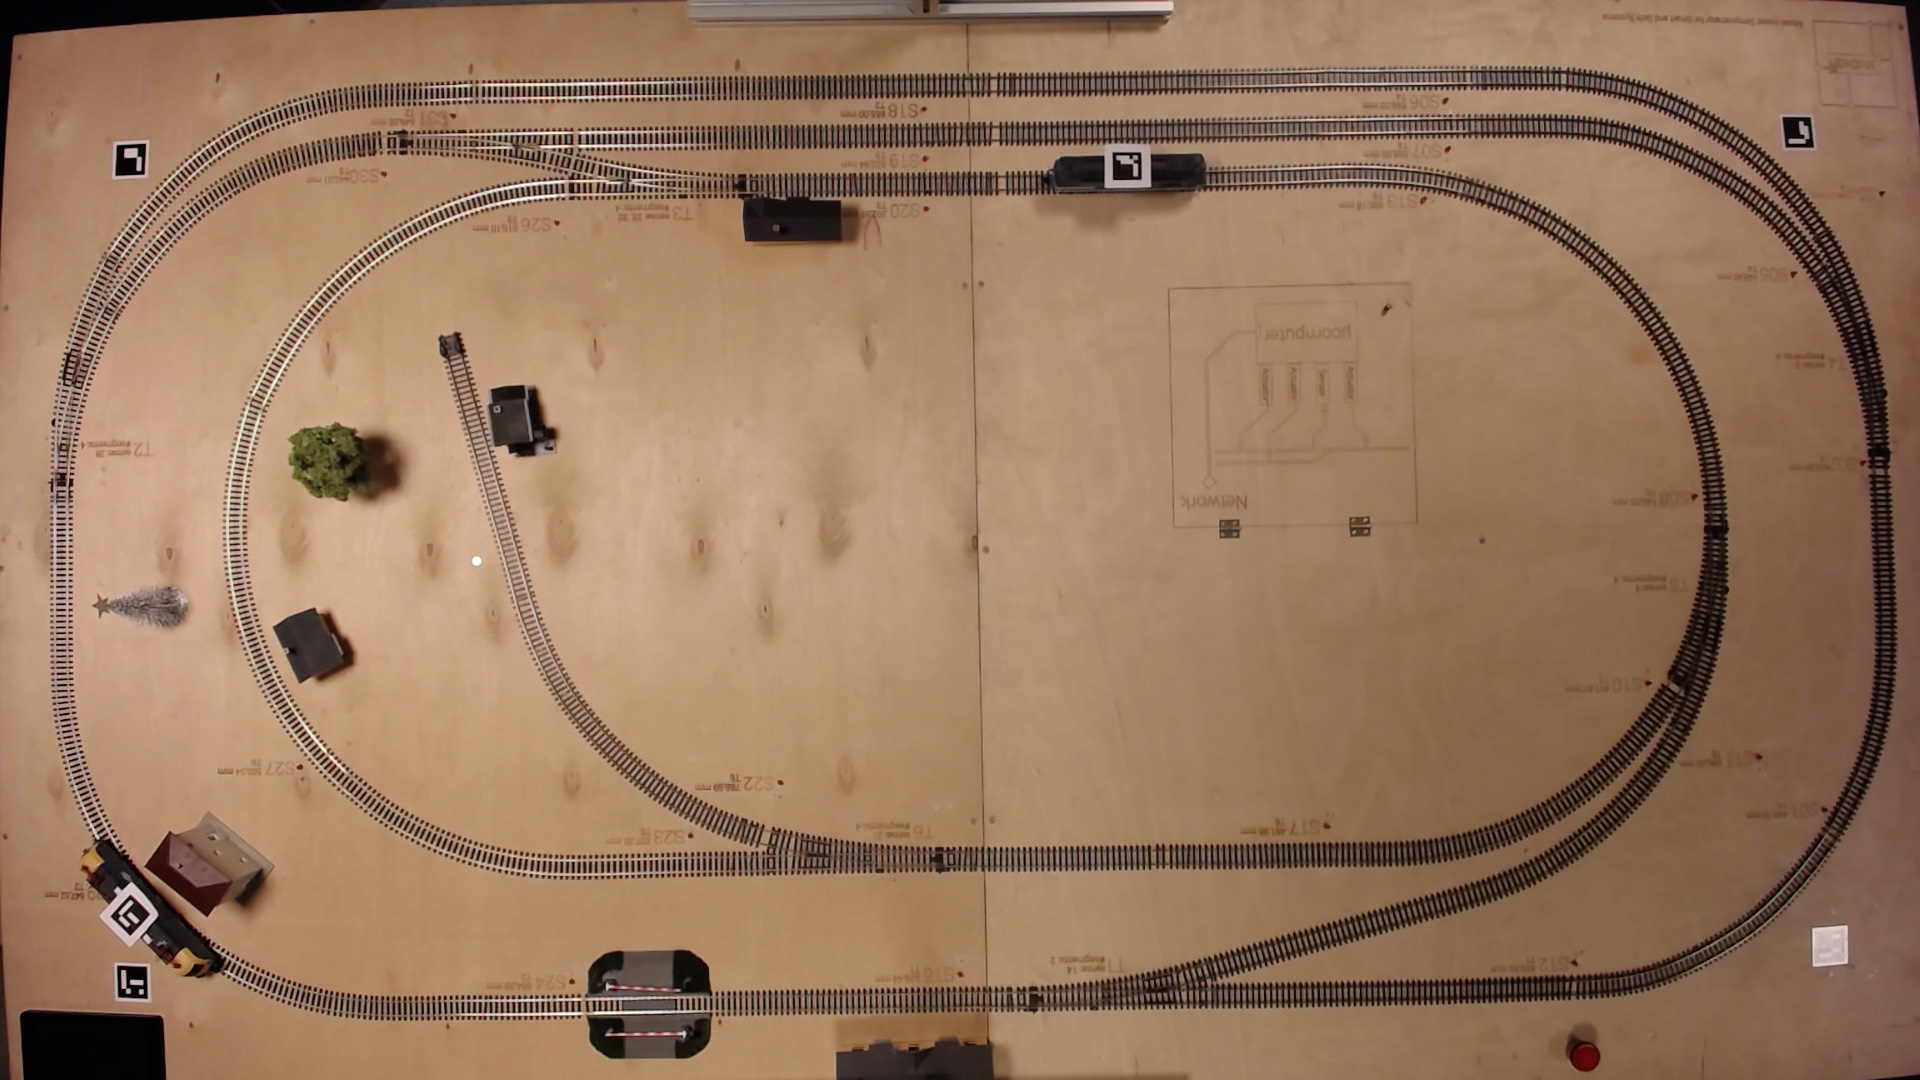
\includegraphics[width=150mm]{figures/modes3/overview.jpg}
	\caption{Railway system overview}
	\label{fig:overview}
\end{figure}
\section{Railway system basic components}
First of all I want to introduce the physical components and the basic process of the railway systems stub. There are 31 sections, with one blind track and 7 turnouts. The \ref{fig:layout} figure shows the layout of the railway elements with corresponding segment ids. Over all a segment means either section or turnout.
\todo[inline]{Create more visible figure about layout}
\begin{figure}[h]
	\centering
	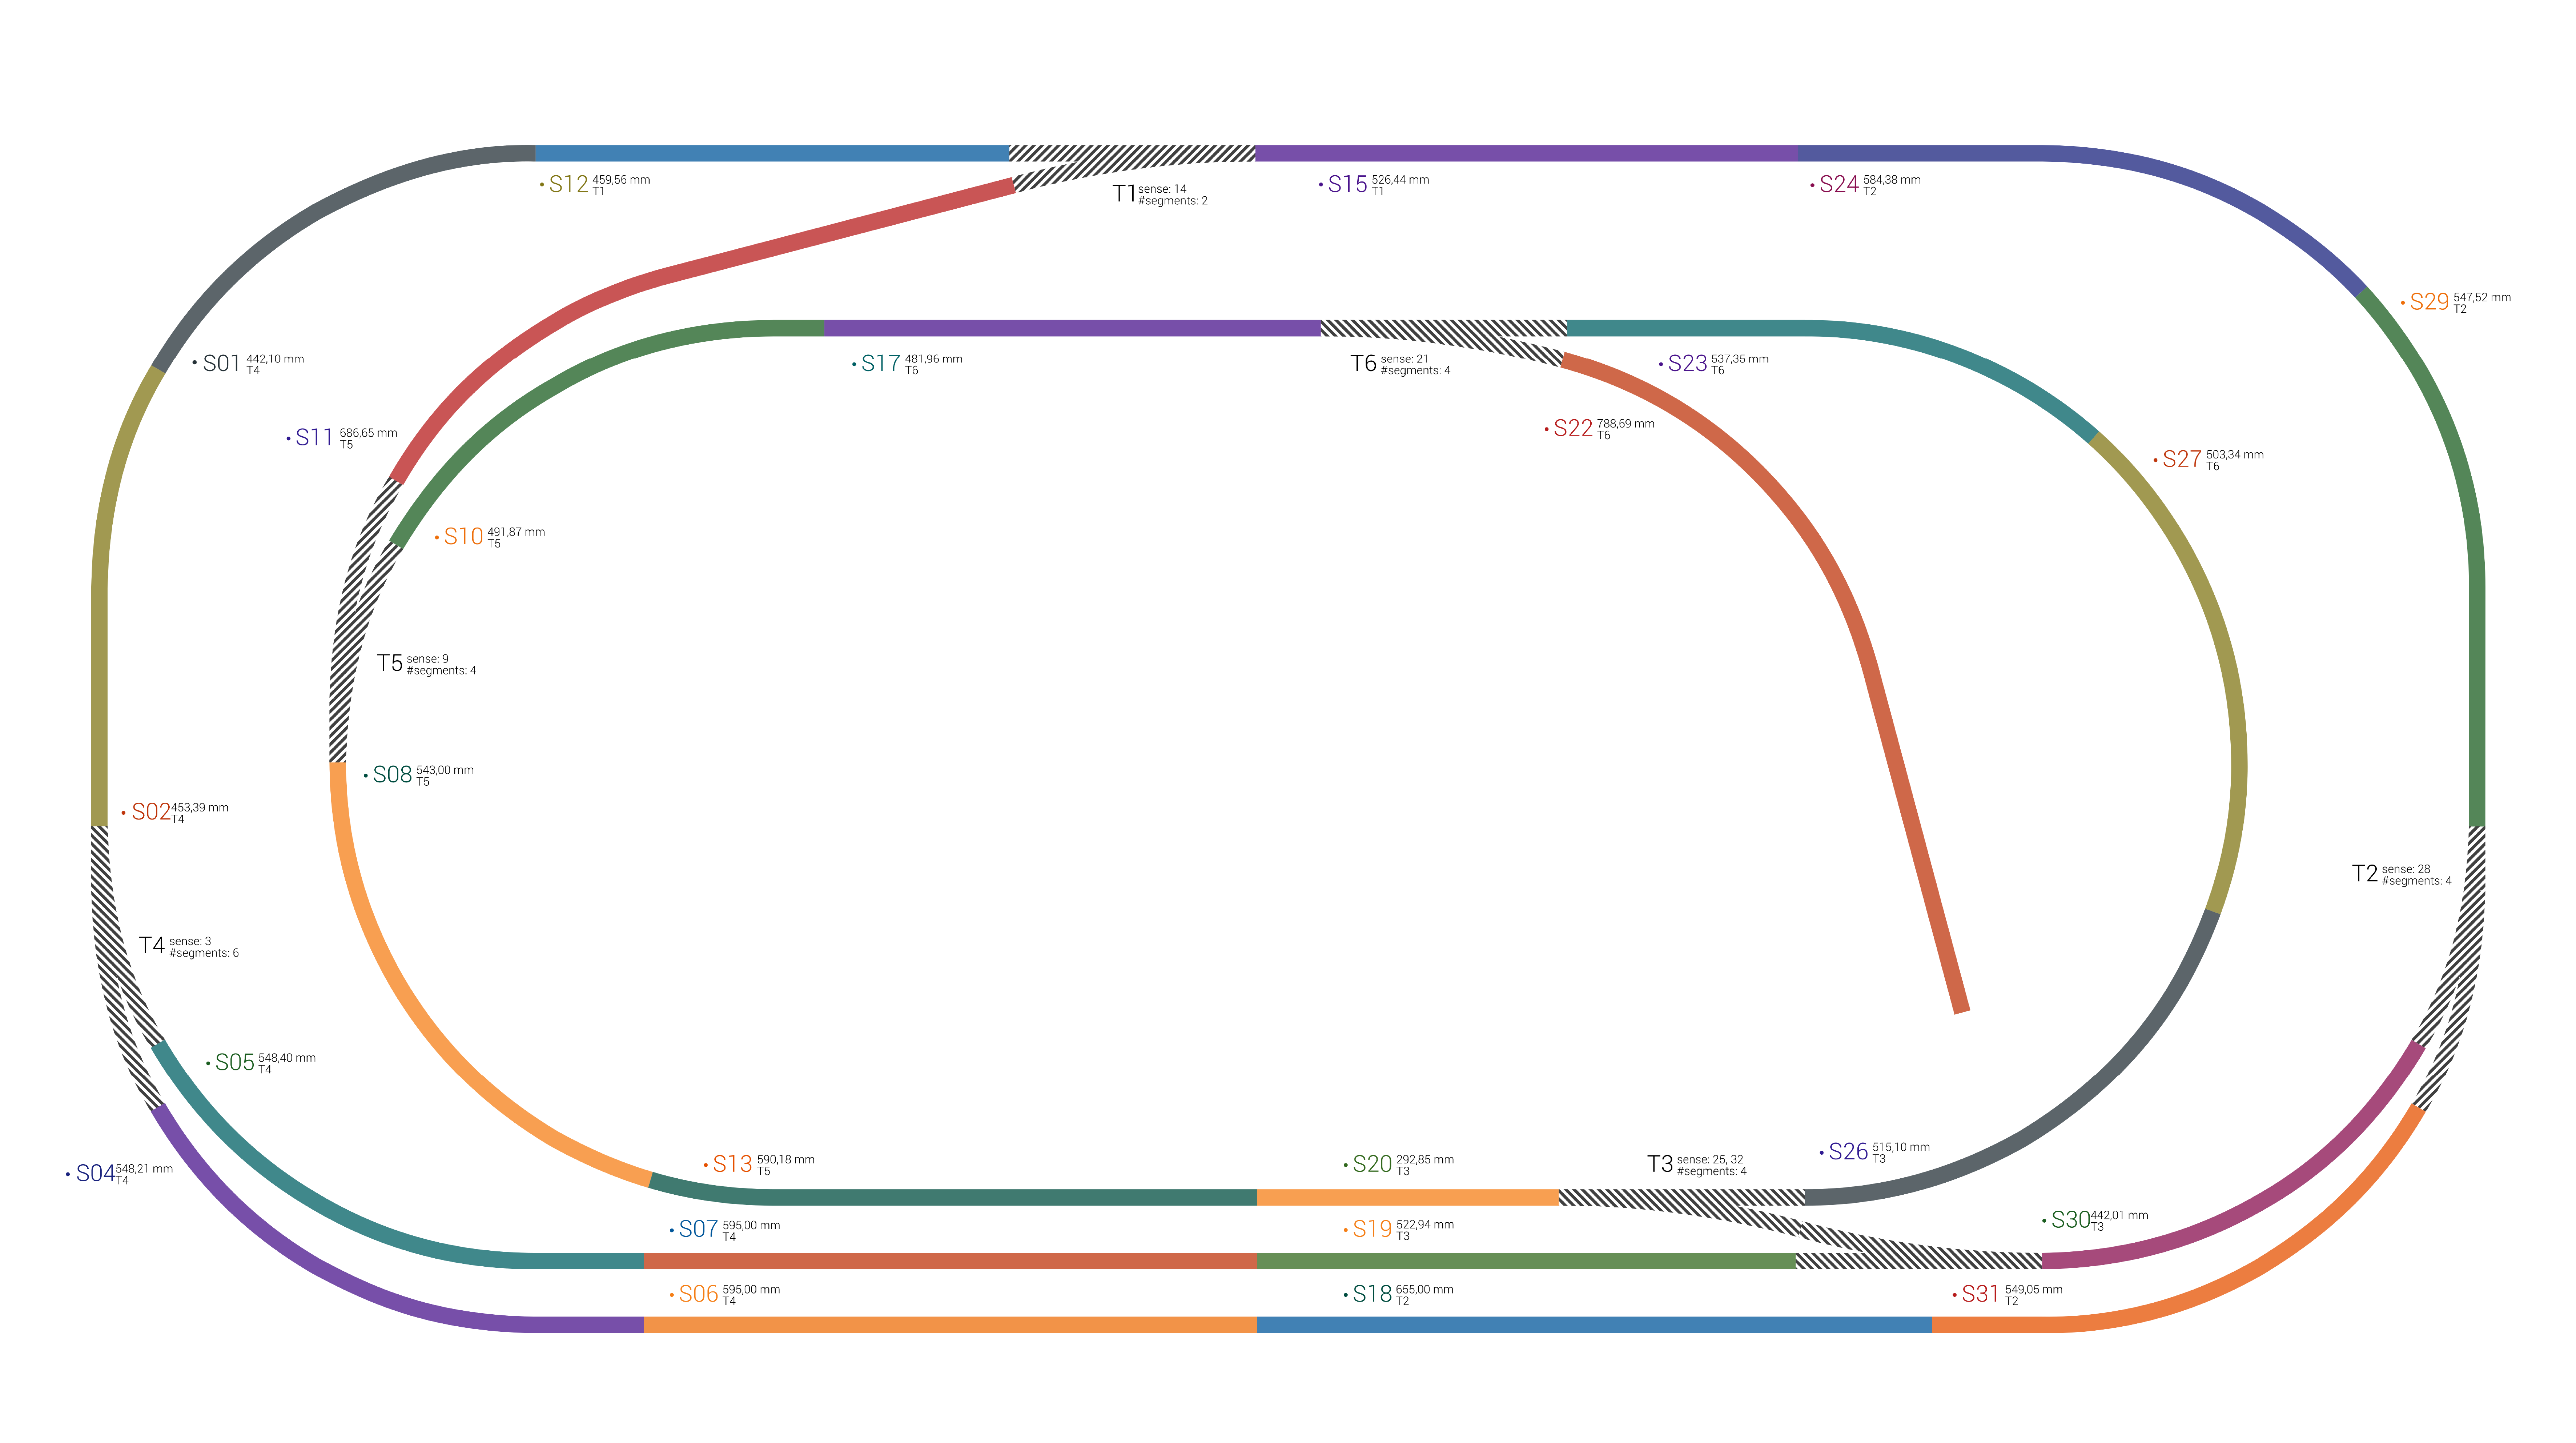
\includegraphics[width=150mm, keepaspectratio]{figures/modes3/layout2.png}
	\caption{Railway layout}
	\label{fig:layout}
\end{figure}
\paragraph{Section} 
First principal  element is a 15-20 cm long railroad. Each section is connected to 2 other sections, and wired to a command station, which gives them sufficient power source for moving the trains on them. In the figure \ref{fig:layout} these sections are identified by \textit{SXX} strings, where \textit{XX} is two unique digits for this layout. Furthermore these numerals determines which bit shows this section's occupancy in the occupancy vector later (see section \ref{section:OccupancyDetection} for more information). On the \ref{fig:layout} figure for each section lengths and responsible BeagleBone Black ids are shown.

\paragraph{Turnout}
Second principal element is the turnout, which can differentiate 2 paths on the track as it can be seen on figure \ref{fig:turnoutDir}. The train which is going through a turnout can reach different sections depending on the state of the turnout. On the layout figure (\ref{fig:layout}) each of these elements are visible as gray dashed sections with the IDs. Each turnout ID starts with T and ends with a numeric (1..6). These IDs determines, which bit identifies the turnout's occupancy in the occupancy vector) and \textit{\#segments} as number of supervised sections by the BeagleBone Black (see section \ref{section:OccupancyDetection} for more information about occupancy vector).
\begin{figure}[!h]
	\centering
	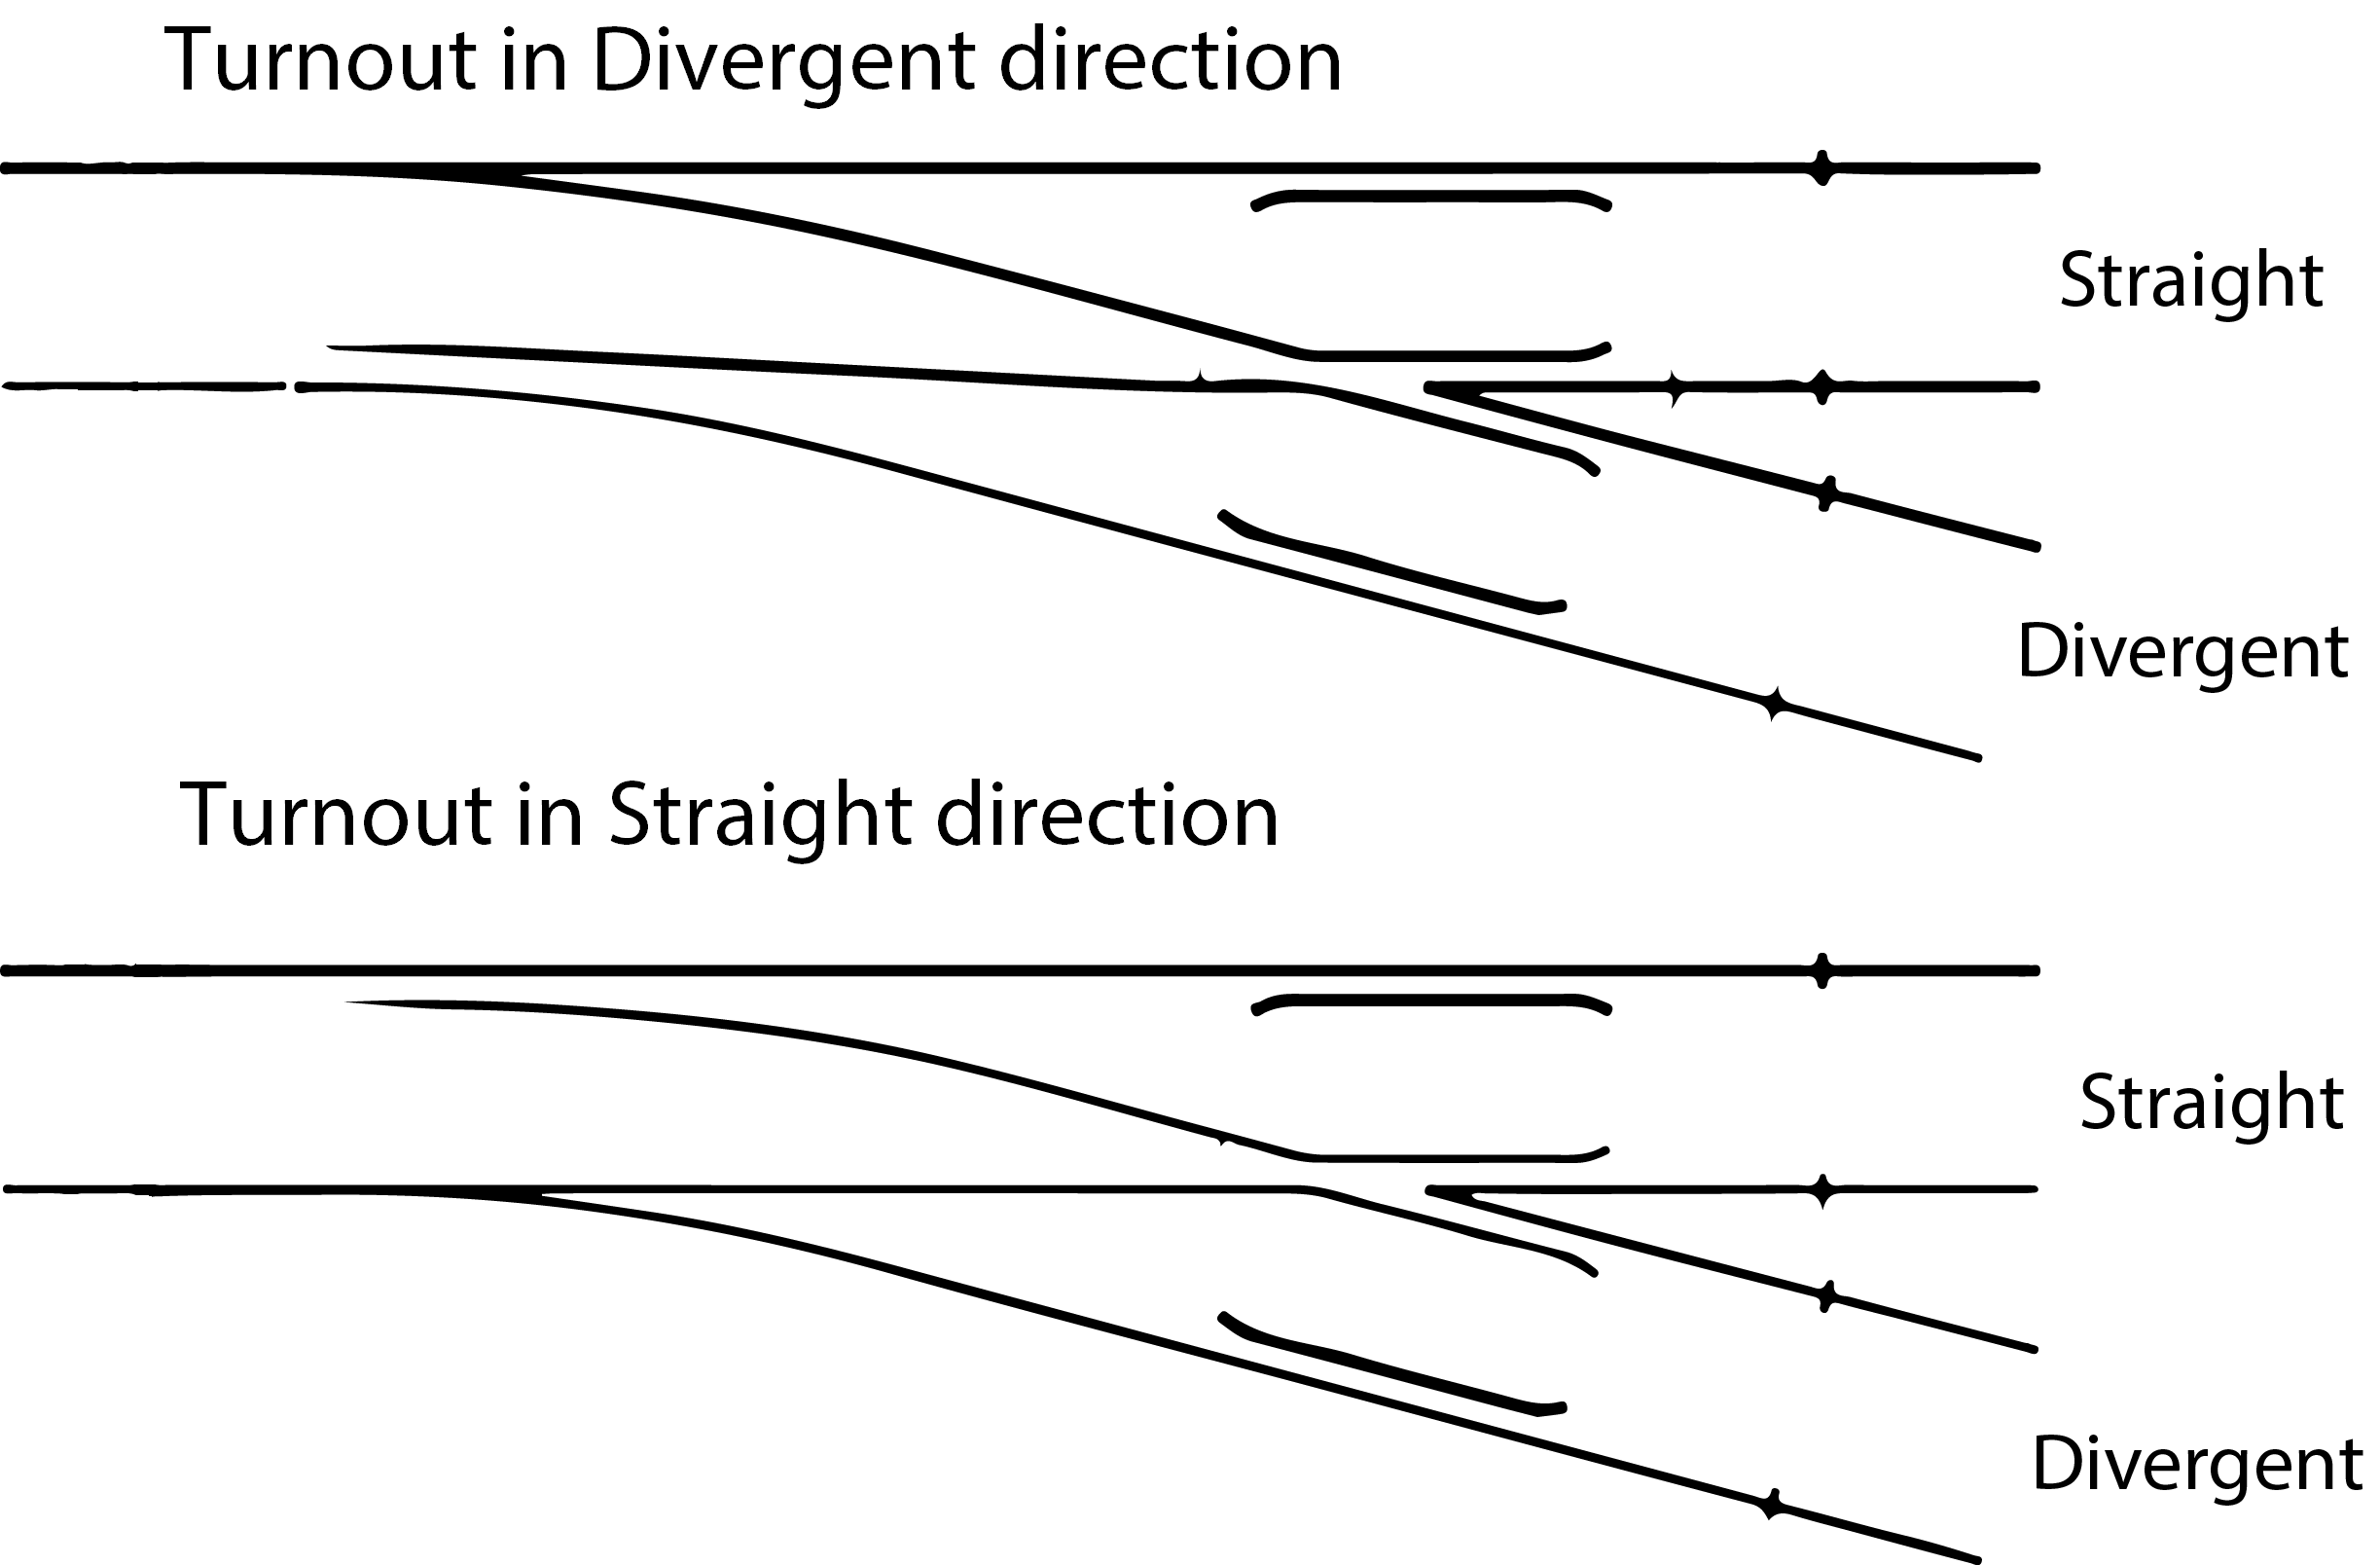
\includegraphics[width=150mm]{figures/modes3/turnout.png}
	\caption{Turnout directions}
	\label{fig:turnoutDir}
\end{figure}

\paragraph{Train} \label{par:trainScenarios}
There are 2 model trains, which can move on the sections and turnouts. The first safety critical paradigm is to avoid a train collision on the track, for which the basic scenarios are the following. 

First approach is that 2 trains are passing through the same turnout, from the same direction on different paths. It means that they are approaching the same section of the turnout, so they will collide like on the \ref{fig:LayoutT1-scenario1} figure.
\begin{figure}[!h]
	\centering
	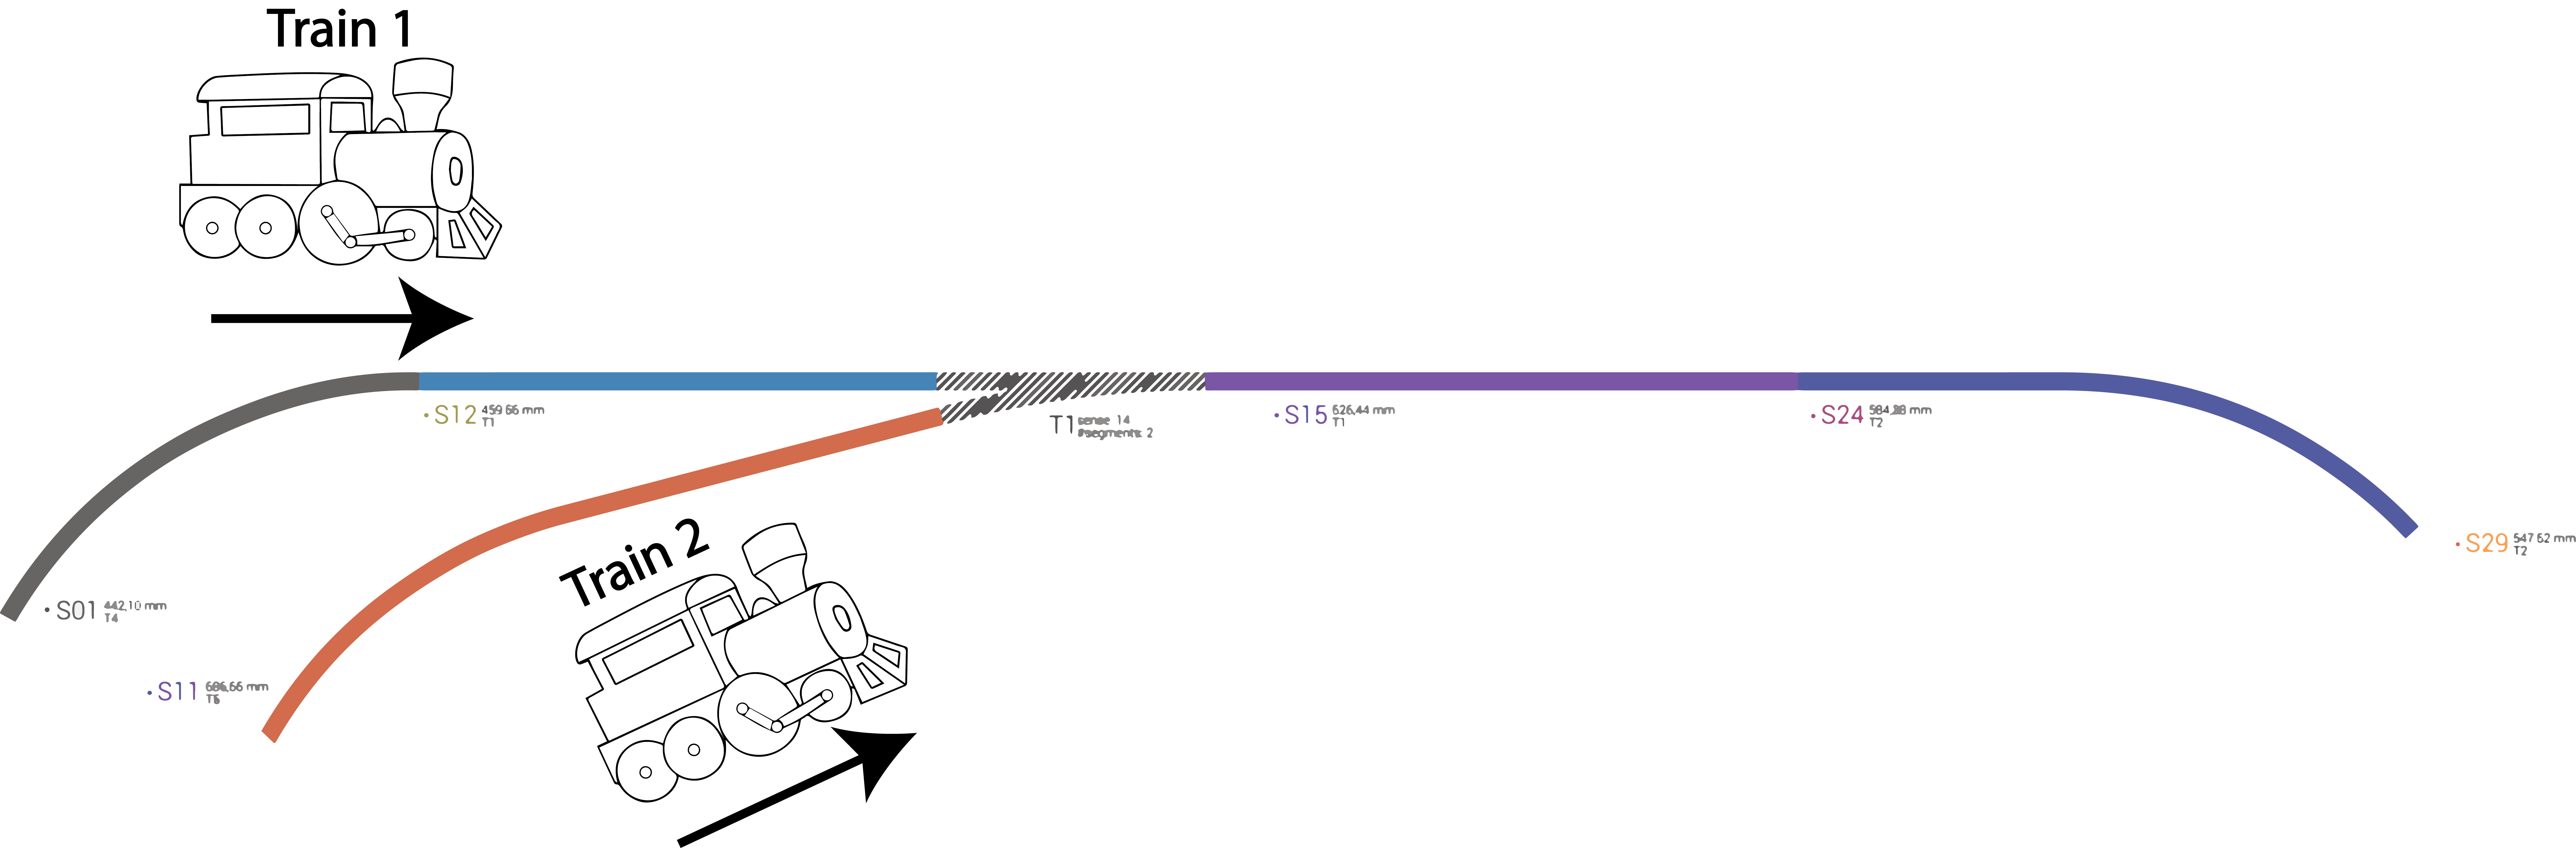
\includegraphics[width=150mm, keepaspectratio]{figures/modes3/layoutT1-scenario1.png}
	\caption{Turnout 1 collision scenario 1}
	\label{fig:LayoutT1-scenario1}
\end{figure}

Next possible scenario is shown in \ref{fig:LayoutT1-scenario2} figure, when \textit{Train 1} is going to the section where \textit{Train 2} is staying. Notice that no matter in which direction the \textit{Train 2} is moving or staying, it is a dangerous situation.
\begin{figure}[!h]
	\centering
	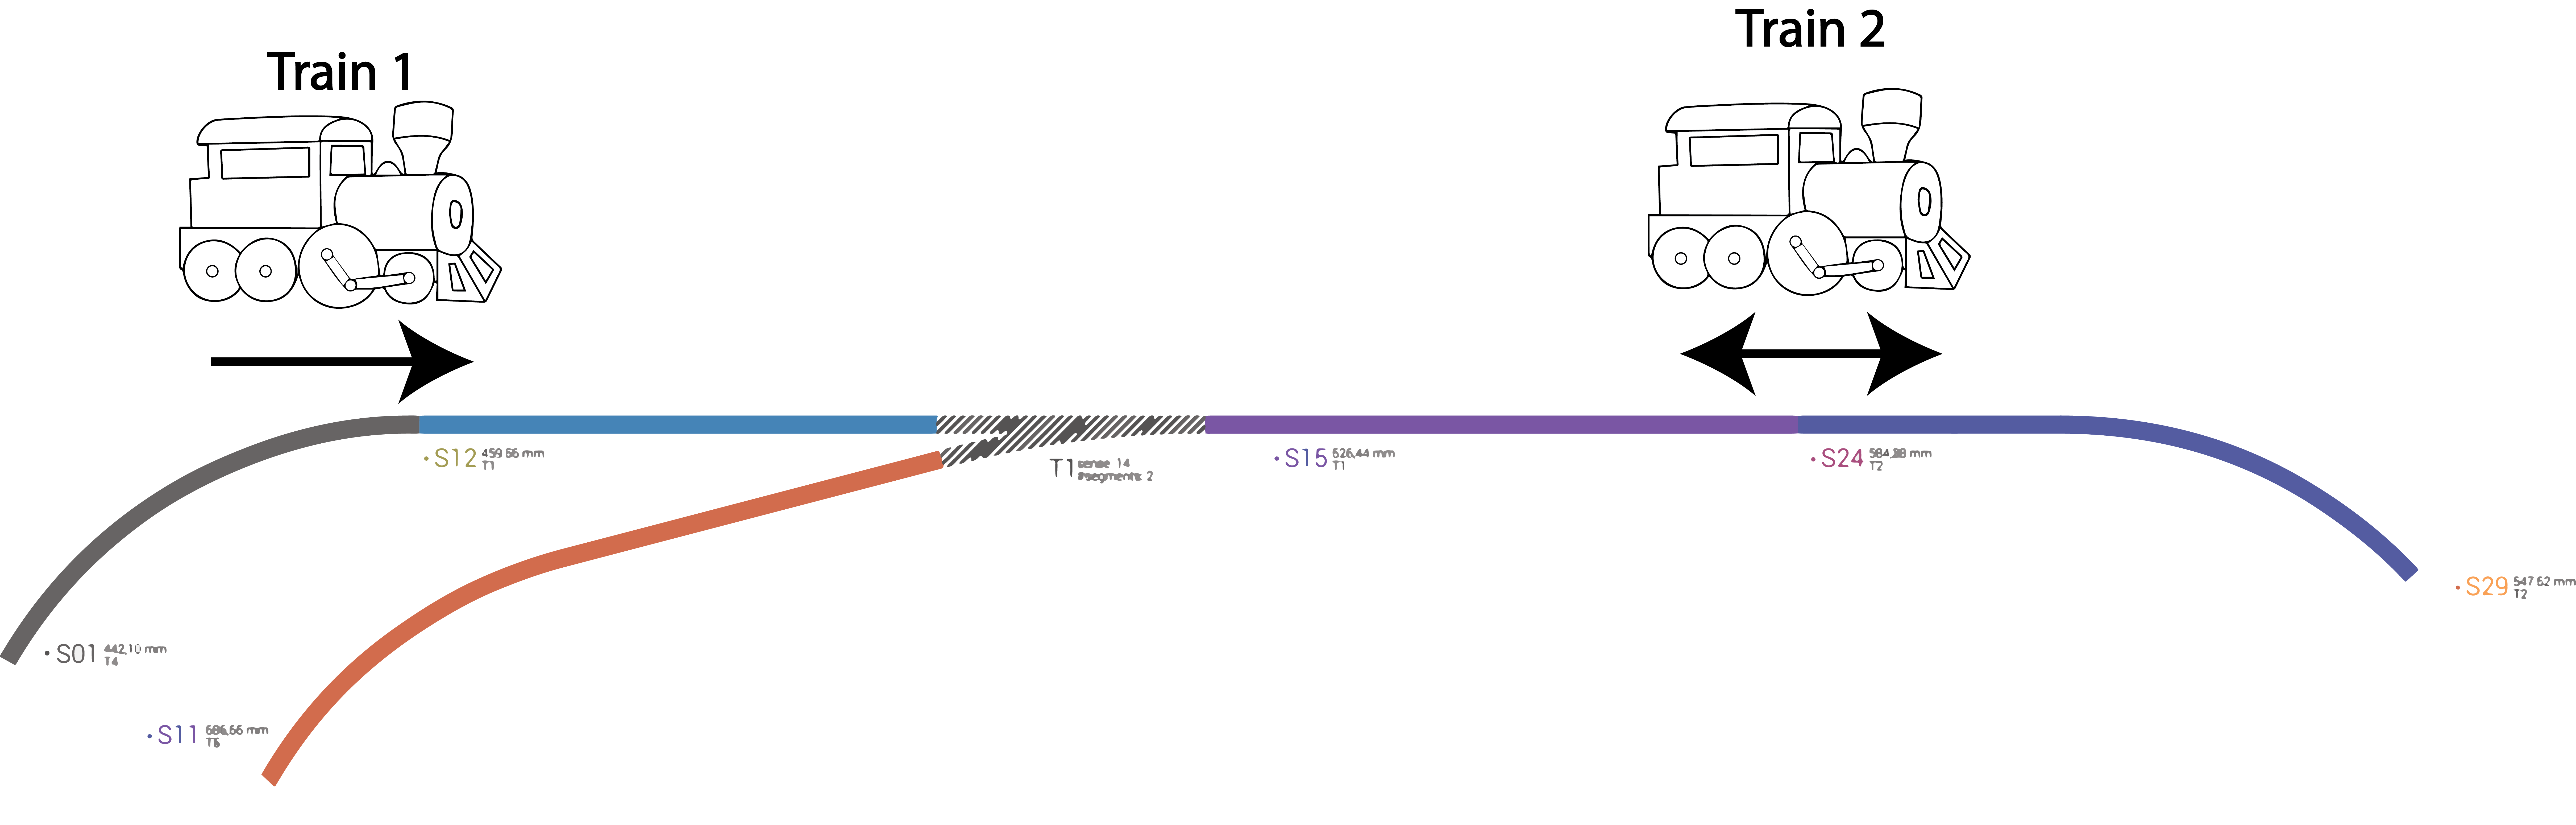
\includegraphics[width=150mm, keepaspectratio]{figures/modes3/layoutT1-scenario2.png}
	\caption{Turnout 1 collision scenario 2}
	\label{fig:LayoutT1-scenario2}
\end{figure}

\paragraph{Command Station}
Supply power source for the sections which provides tension for the trains on the track.

\paragraph{Controller}
In connection with the \textit{Command Station} an XPressNet protocol \footnote{More details about XPressNet Protocol \url{http://www.lenzusa.com/1newsite1/Manuals/xpressnet.pdf}} based controller is attached to the system. This component's purpose is setting the direction and speed for each train on the track through the \textit{Command Station}.

\section{Hardware extensions}
The basic hardware environment is not sufficient for controlling and analyzing purposes, therefore additional hardware elements have been designed for that. These platforms are also custom made and also off-the-shelf products. 
\todo[inline]{Check if these infos are belong to here}
For modeling purposes I have used MagicDraw with Sysml plugin \cite{SysML}.
The \ref{appendix:HWPictures} appendix contains pictures about the hardware elements.
\subsection{Data processing units}
\begin{figure}[h]
	\centering
	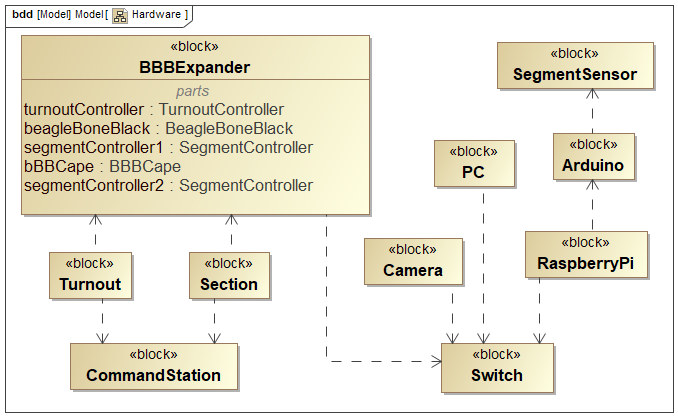
\includegraphics[width=150mm]{figures/modes3/Hardware.png}
	\caption{Hardware block definition diagram}
	\label{fig:Modes3HWBDD}
\end{figure}

\paragraph{BeagleBone Black (BBB)}
An industrial microcontroller platform and it provides 4GB 8-bit eMMC on-board flash storage and 2x PRU 32-bit microcontrollers, which could satisfy the function for parallel monitoring. There are 6 BBB on the track connected to the railway, used for controlling and enabling/disabling each section.

\paragraph{Rapsberry Pi 3}
A Rapsberry Pi microcontroller is dedicated to handle most of the software components related to the Railway demonstrator system. It has twice as large computing capacity in RAM and also in CPU as BBB.

\paragraph{Arduino}
Dedicated hardware element for reading from the 6 DigiSens-8-S88 output data through S88 protocol (see \ref{par:SegmentSensor} section for details about this component). This communication layer requires proper timing conditions which the Arduino platform can satisfy.

\subsection{Custom hardware extensions}
\paragraph{BeagleBone Black cape and expanders}\label{par:BBBcape}
The BeagleBone Black components expect 5VDC power source instead of 12VDC which our power station supplies. Because of that reason a so called cape have been created for each controller. Additionally the need for easy-to-use ports to attach additional circuits to the main board also have come up. The expanders could be used to extend the functionality of one BeagleBone unit, which is on the figure \ref{fig:capeSysml}. 

\begin{figure}[!h]
	\centering
	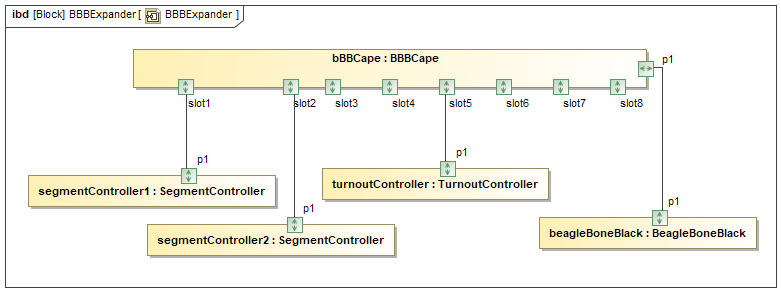
\includegraphics[width=150mm]{figures/modes3/BBBExpander.png}
	\caption{Layout and current attachment of cape and expander}
	\label{fig:capeSysml}
\end{figure}

Each cape have 8 general purpose expander slot, for which the pin layout is expressed in the following \ref{table:expander_pin_layout} table.

\begin{table}[!h]
	\caption{Pin layout}
	\label{table:expander_pin_layout}
	\begin{center}
		\renewcommand{\arraystretch}{1.5}
		\begin{tabu} to 0.5\textwidth { | X[c] | X[c] | X[c] | X[c] |}
			\hline
			G3 & G2 & G1 & G0 \\
			\hline
			3V3  & 5V  & Gnd  & 12V\\
			\hline
		\end{tabu}
	\end{center}
\end{table} 
\url{https://github.com/FTSRG/BME-MODES3/wiki/HW-Expander-design#gpio-basic-usage}
\todo[inline]{Give proper details about G0-G15 pins, the table is not showing all of them like} 
The upper row of each connector is dedicated for GPIO connections. Two of the GPIO pins connected to the application processor (labeled with G0..G15), and the remaining two GPIO pins are connected to the PRU unit (labeled P0..P15).

With this setup, the PRU and the application processor can cooperate on hardware level.

\paragraph{Segment sensor}\label{par:SegmentSensor}
 The DigiSens-8-S88 component is an off-the-shelf product, which can detect the occupancy for 8 segments.\footnote{More information about the product can be found here:\url{http://www.digitools.hu/termekek/erzekelok/digisens-8-s88}}.

\paragraph{Segment actuator}
Segment Actuator expanders are designed to stop a train on the corresponding segment. The concept behind this expander based on the Lenz Asymmetrical DCC and ABC functionality of train-decoders. \footnote{The following descriptions are based on \url{https://tonystrains.com/lenz-asymmetrical-dcc-and-abc/} article.}

ABC (Automatic Brake Control) works in conjunction with Asymmetrical DCC. Asymmetrical DCC is a way to trigger ABC in the decoder. This gives the ability to stop trains at a section of the track with Asymmetrical DCC.

\begin{figure}[!h]
	\centering
	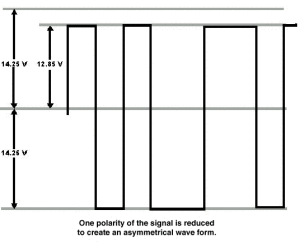
\includegraphics[width=100mm]{figures/modes3/DCC.png}
	\caption{Asymmetric DCC voltages}
	\label{fig:dcc}
\end{figure}

The Asymmetrical DCC signal is generated by offsetting one phase of the DCC signal. This signal then triggers the Automatic Brake Control in the decoder. This causes the engine to stop at the distance set up in the Constant Stopping Distance feature. We implemented this using five diodes. %connected in the form as shown in the figure below.
%\begin{figure}[h]
%	\centering
%	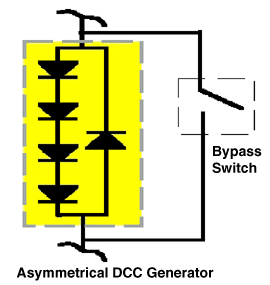
\includegraphics[width=50mm]{figures/modes3/abc.png}
%	\caption{Asymmetric DCC voltages}
%	\label{fig:abc}
%\end{figure}

The Segment Actuators uses this setup and also gives an interface (with GPIOs) to enable or disable this feature. Every Segment Actuator expander has two slots (A or B) and can enable or disable two segments. Each segment can be enabled setting two GPIOs to HIGH level, one connected to the PRU and one connected to the application processor.

\paragraph{Turnout actuator}
Turnout Actuator expanders can switch turnouts on the table between their states. Previously, we have managed to solve this with COTS units, but in that case we were not able to query the position of the switch programmatically. This expander gives the ability for both switching the turnout and sensing its state.

The concept behind this unit is based on the fact, that turnout mechanism is working as an wire between the common (COM) pole and an other pole (STR or DIV) when switched in one position, therefore we can sense its state.

The electronic characteristics of the BeagleBone unit could not satisfy the switching process electrically, thus we had to use a micro-controller (an Atmega328 MCU). Also, the state-sensing process is based on Analog to Digital Converters, which are also integrated into the MCU.

\textbf{Usage}
The MCU has 2 inputs and 2 outputs connected to the expander connector as shown in the table below.
\begin{center}
	\renewcommand{\arraystretch}{1.5}
	\begin{tabu} to 1.0\textwidth {X[c] X[c] X[c] X[c]}
		\toprule
		Pin 0                                  & Pin 1                                   & Pin 2                           & Pin 3                             \\ \midrule
		Turnout switching to Straight position & Turnout switching to Divergent position & Turnout state sensing (Straing) & Turnout state sensing (Divergent) \\
		INPUT for the MCU                      & INPUT for hte MCU                       & OUTPUT for the MCU              & OUTPUT for the MCU                \\ \bottomrule
	\end{tabu}
\end{center}


\section{Software components}

\begin{figure}[h]
	\centering
	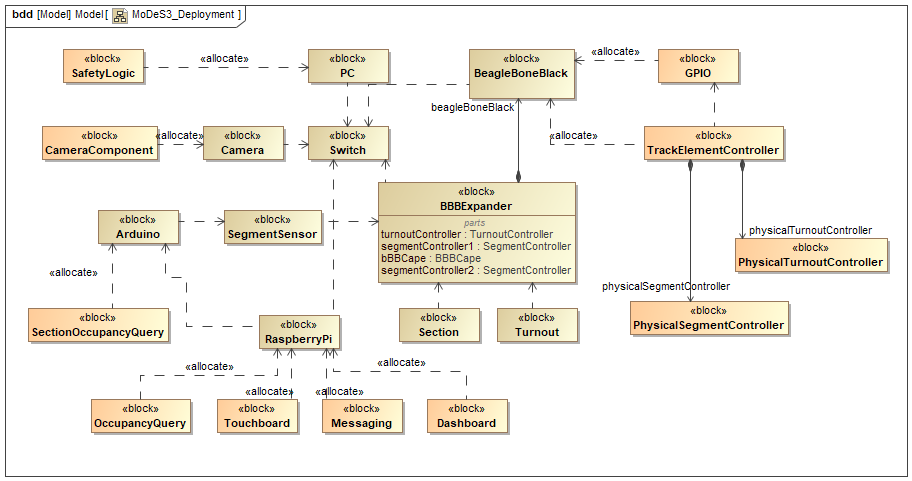
\includegraphics[width=150mm]{figures/modes3/MoDeS3_Deployment1.png}
	\caption{Software components deployment to hardware elements}
	\label{fig:Modes3Deployment}
\end{figure}
\subsection{Occupancy detection elements} \label{section:OccupancyDetection}
\paragraph{Section Occupancy Query}
Responsible for debouncing the 32bit long occupancy vector with proper timing conditions regarding S88 protocol and forward this 32bit to \textit{Occupancy Query} through usb connection. Computed data contains the occupancy information for each track element (section or turnout) per one bit.
\paragraph{Occupancy Query}
In connection with the \textit{Section Occupancy Query} process the occupancy state for the whole track. Only if the state has changed, it sends occupancy change message to the MQTT topic with the track element id and new occupancy state.

\subsection{Track element control elements}
\paragraph{GPIO}
Handle the GPIO pin changes and commands for each extension point of the BBB cape (see \ref{par:BBBcape} section for details about BBB cape and expanders).
\paragraph{Physical Segment Controller}
For each segment there are two GPIO instance to serve the control mechanism of application and the PRU also, however there is no PRU control implemented.
\paragraph{Physical Turnout Controller}
For each turnout controller, there are four GPIO pins: two for control the turnout itself (straight and divergent direction), and other two to get info about the current state.
\paragraph{Track Element Controller}
Implementation of the platform-specific actuator code of disabling and enabling sections and setting turnout directions for the BeagleBone Black embedded units.

\subsection{Track control and supervisor elements}
\paragraph{XPressNet}
Protocol for sending messages to the \textit{Command Station} component, therefore we can extend to communication form for controlling the track. In the current layout there is a controller and web-based opportunity for controlling.
\paragraph{Dashboard}
Model railway track dashboard implementation. In Addition this component is instantiated only once, and up for the whole time while the track is in use. Consequently we can reach one common dashboard from the web and it contains the actual occupancy and track element status.
\paragraph{Touch board}
Dashboard for the model railway track, with focus on touchable elements, that can be controlled.
\paragraph{Safety Logic}
In the MODES$^3$ safety critical project we want to avoid the collision of model trains, therefore the safety logic software component detects these critical scenarios by Viatra Query \cite{Viatra} patterns and act the necessary action (for example disable a section).


\subsection{Messaging elements}
Each software component share information about the railroad system through the messaging software element, which is based on protobuf messages and provides high-level designed API with MQTT for this purpose. 
\begin{figure}[!h]
	\centering
	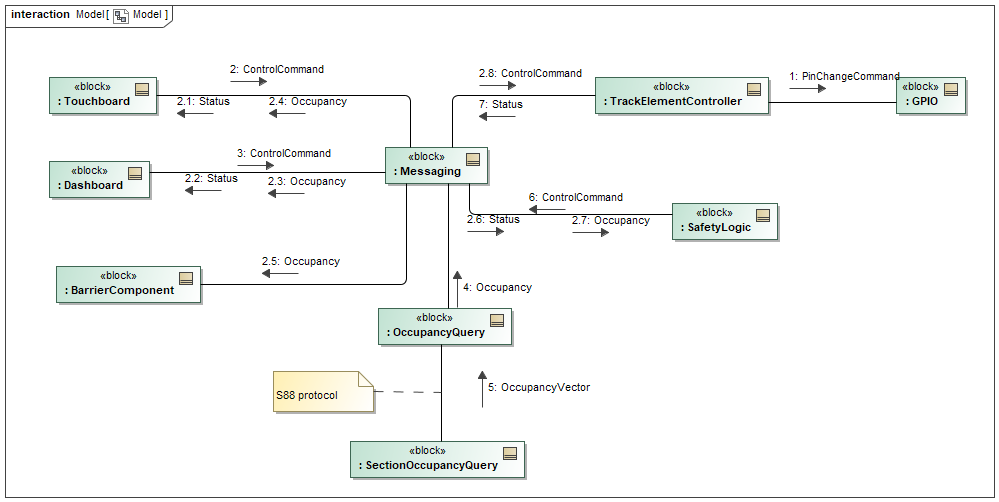
\includegraphics[width=150mm, keepaspectratio]{figures/modes3/CommunicationModel.png}
	\caption{Communication between software components}
	\label{fig:communicationModel}
\end{figure}

Separated topics are created for different information flow, and any component can subscribe for these topics. Basically on all topic, the information reporting is change based, so all components sending an information message to the dedicated topic when their state have changed (like occupancy changed or turnout changed). In opposite to that, there is a \textit{SendAllStatusCommand} and for that every component should send the actual status.

I will now list the specific MQTT topics and the connected software components to that, so basically what kind of information is flowing on them. (See software component connections on figure \ref{fig:communicationModel})

\paragraph{Segment Occupancy topic}
On this topic the \textit{Occupancy Query} component sending information whether an occupancy state is changed on any segment. (Notice that a segment can also be a section ot a turnout too.) Most of the components are subscribed for this information topic so the \textit{Touch board}, \textit{DashBoard}, \textit{Barrier} (only for the supervised segments), \textit{Track Element Controller} and \textit{Safety Logic}.

\paragraph{Segment and Turnout Command topic}\label{par:MQTTTopicCommand}
Basically the \textit{Track Element Controller} process and accomplish these commands, and \textit{Touch board}, \textit{Dashboard} and \textit{Safety Logic} components can give these instructions.

\paragraph{Segment and Turnout Status topic}\label{par:MQTTTopicStatus}
For every command the \textit{Track Element Controller} will give a status acknowledgement message with the new state of the turnout or section. In this way the \textit{Touch board}, \textit{Dashboard} and \textit{Safety Logic} elements will be informed about the latest and current state.

\paragraph{CV topic}
The camera notification is communicated on that topic, which is received by the \textit{Safety Logic}.

\paragraph{ALL topic}
For this specific topic all the components in the system are subscribed, and information about train controlling and \textit{Command Station} related messages are shared.

\subsection{Complementary elements}
\paragraph{Barrier} 
Sends open/close commands to the barrier over the network, depending on the occupancy of supervised segments.
\paragraph{Leapmotion}
Software component for converting gestures into special movements for changing the speed of a specific train.

\section{Components by functional purpose}
%\todo[inline]{Maybe figure of the Sw-Hw sysml for each paragraph}
\paragraph{Occupancy detection}\label{par:FunctionOccupancyDetection}
In order to know where are the trains on the track, we first must know which track elements (section or turnout) is occupied. This attribute can be determined whether the specific section has power consumption, which is used by train on it. The actual detection is made by the\textit{ DigiSens-8-S88} sensing element. The demonstration railway system have four sensing element, and they are connected to an\textit{ Arduino} S88 port. This microcontroller computes a basic low-level calculation by \textit{Section Occupancy Query} C++ software component and forwards the 32-bit occupancy information (actual state of every track element) to the \textit{Occupancy Query} via USB. The\textit{ Occupancy Query} Java component on the \textit{Rapsberry Pi} stores the previous occupancy state, and sends information to the \textit{Segment Occupancy} topic.

\paragraph{Track element controlling}\label{par:FunctionTEC}
For safety critical purposes in any collision scenario it is a good manner to disable all track elements, which is affected in the critical scenario. To make this switch possible, we have to cut the electric circle between the segment and \textit{Command Station}. The \textit{Section Controller} hardware element have been developed for changing a section, consequently the \textit{Turnout Controller} is responsible for changing a turnout. These hardware elements are attached to a \textit{BBB cape}, which is designed for supplying extension ports for BBB. In software point of view, through GPIO pins (specific file writing), we can give impulses from the BBB to the section or turnout. Therefore a \textit{GPIO manager} component is responsible for that in connection with the \textit{Track Element Controller component}. Both of them are Java components and deployed to the BBB microcontrollers.

\paragraph{Safety critical verification}
Because of the network communication, it is easy to connect a \textit{safety logic} in the system. In addition a camera component is reading the position of the trains on the track. If the \textit{Safety Logic} detects an unsafe scenario from the occupancy detection or camera, it switches off the affected elements by a \textit{Track Element Controller} signal.
